\subsection{Pushbutton KEY and LED Port}
\label{sec:hps_gpio1}
The HPS includes a general purpose I/O port, called {\it GPIO1}, that is accessible by the
ARM A9 processor.  As illustrated in Figure~\ref{fig:gpio1}, this parallel 
port is assigned the {\it Base} address {\sf 0xFF709000}, and includes several 32-bit registers.
These registers can be read or written using word accesses.
Only two bit locations in GPIO1 are used for the \systemName. Bit~24 of the data
register (DR) is connected to
a green light, LEDG, and bit~25 is connected to a pushbutton switch, KEY. To use these
devices, the {\it data direction register} (DDR) shown in the figure has to be configured such 
that bit~24 is an output and bit~25 is an input. Writing a 1 into a corresponding bit
position in the DDR sets this bit as an output, while writing a 0 sets the bit as an
input. After the direction bits have been set, the green light LEDG can be turned on/off 
by writing to bit~24 in the data register. The
value of the pushbutton switch KEY can be obtained by reading the external port register
and checking the value 
of bit~25. An example program for the ARM A9 processor that uses GPIO1 is given in Section
\ref{sec:timers}.

As indicated in Figure~\ref{fig:gpio1}, the GPIO1 port includes several other registers in
addition to the DR and DDR registers. These other registers are mostly used for setting
characteristics of input pins, which affects only the KEY input in our system.
Detailed information about these registers can be found in the {\it Cyclone V Hard 
Processor System} documentation, which is available on the Internet.

\begin{figure}[h!]
   \begin{center}
       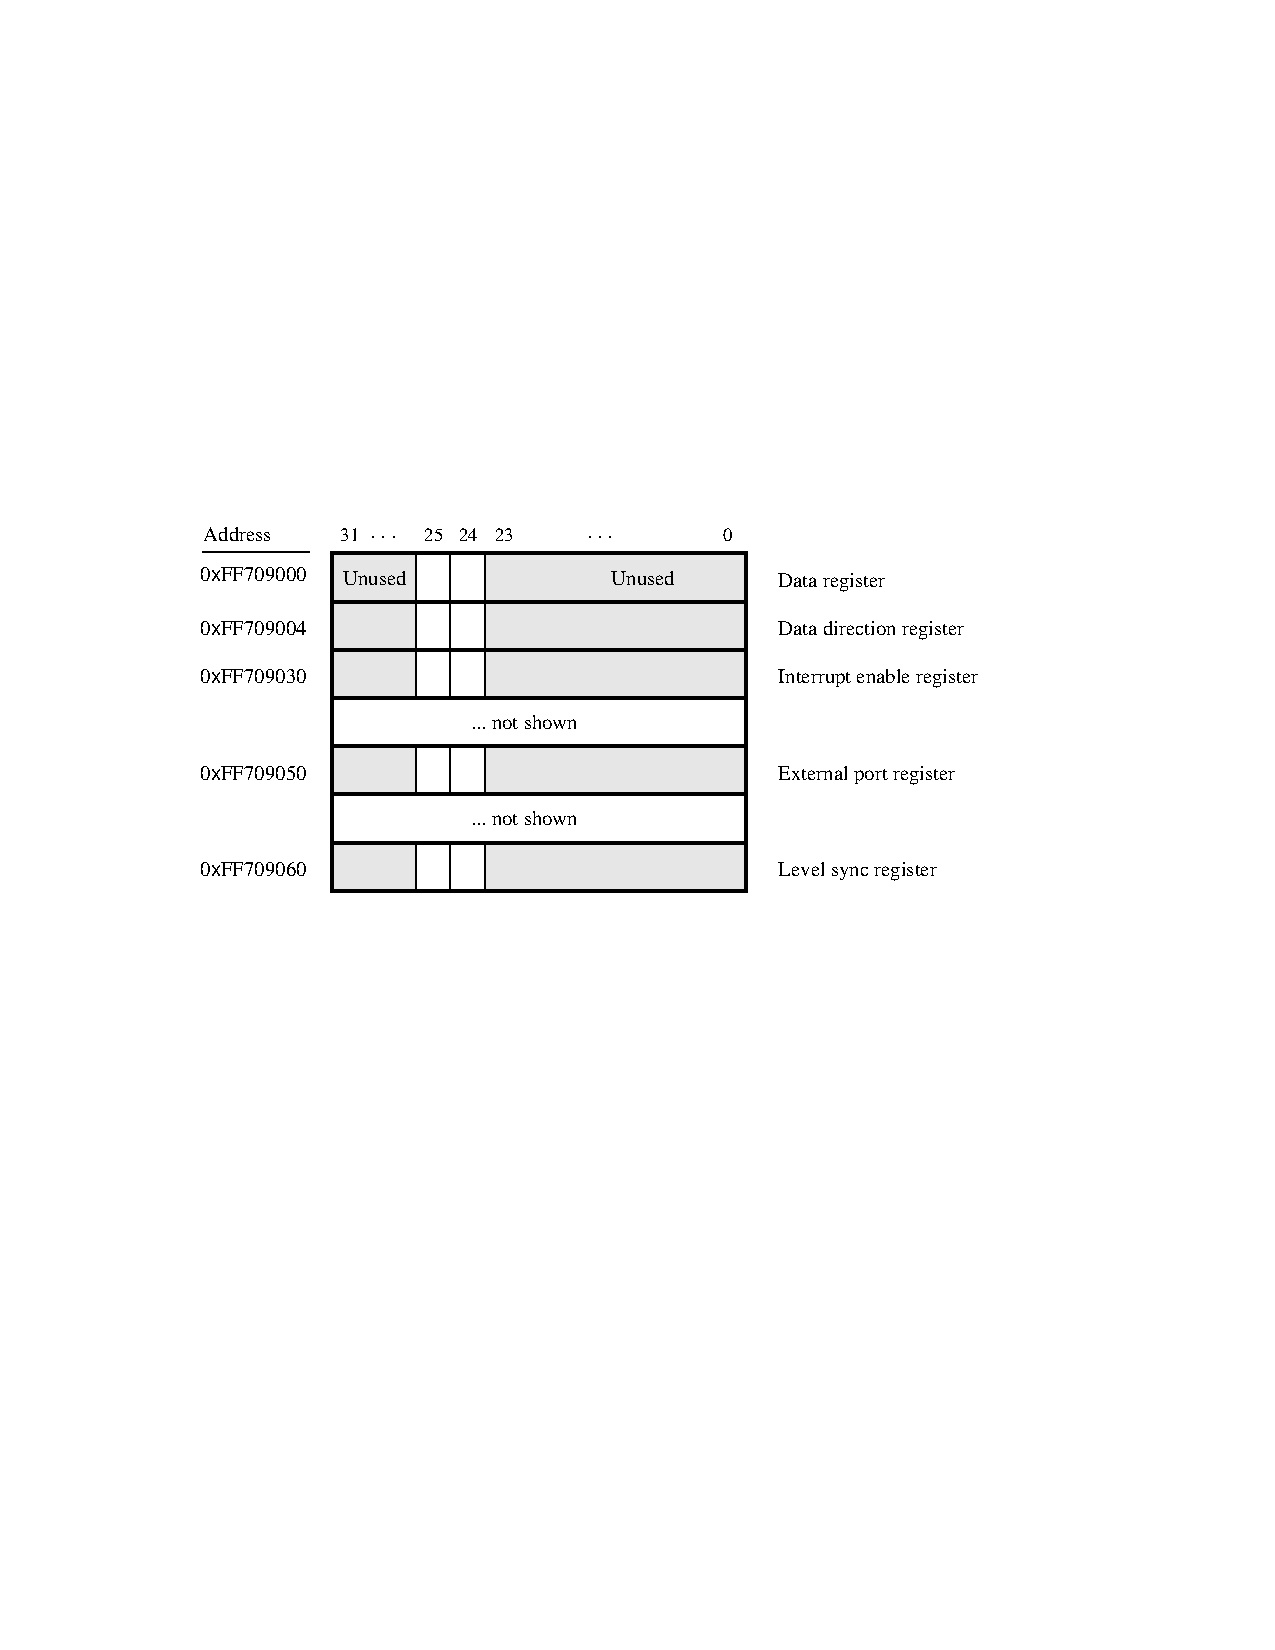
\includegraphics{../../../common/figs/HPS_GPIO1.pdf}
   \end{center}
   \caption{Parallel port GPIO1.}
	\label{fig:gpio1}
\end{figure}
